\documentclass[ignorenonframetext, professionalfonts, hyperref={pdftex, unicode}]{beamer}
%\usepackage{beamerthemesplit}

\geometry{paperwidth=140mm,paperheight=105mm}

%Hack to specify beamer folder https://tex.stackexchange.com/questions/275600/beamer-themes-on-custom-folder
\makeatletter
  \def\beamer@calltheme#1#2#3{%
    \def\beamer@themelist{#2}
    \@for\beamer@themename:=\beamer@themelist\do
    {\usepackage[{#1}]{\beamer@themelocation/#3\beamer@themename}}}

  \def\usefolder#1{
    \def\beamer@themelocation{#1}
  }
  \def\beamer@themelocation{}
\makeatother
%Packages to be included

\usepackage{graphicx}



\graphicspath{{./branding/}}
\usefolder{./branding}
\usetheme{Promwad}
%\usecolortheme{wolverine}


\usepackage[russian]{babel}
\usepackage[utf8]{inputenc}
\usepackage[T1]{fontenc}

%\usepackage[orientation=landscape, size=custom, width=16, height=9, scale=0.5]{beamerposter}

\usepackage{textcomp}


\usepackage{ulem}

\usepackage{verbatim}

\usepackage{ucs}


\usepackage{listings}
\lstloadlanguages{bash}

\lstset{escapechar=`,
	extendedchars=false,
	language=sh,
	frame=single,
	tabsize=2, 
	columns=fullflexible, 
%	basicstyle=\scriptsize,
	keywordstyle=\color{blue}, 
	commentstyle=\itshape\color{brown},
%	identifierstyle=\ttfamily, 
	stringstyle=\mdseries\color{green}, 
	showstringspaces=false, 
	numbers=none, 
%	numberstyle=\tiny, 
	breaklines=true, 
	inputencoding=utf8,
	keepspaces=true,
	morekeywords={u\_short, u\_char, u\_long, in\_addr}
	}

\definecolor{darkgreen}{cmyk}{0.7, 0, 1, 0.5}

\lstdefinelanguage{diff}
{
    morekeywords={+, -},
    sensitive=false,
    morecomment=[l]{//},
    morecomment=[s]{/*}{*/},
    morecomment=[l][\color{darkgreen}]{+},
    morecomment=[l][\color{red}]{-},
    morestring=[b]",
}

\author[Promwad]{{\bf Promwad}}

%\institution[EPAM]{EPAM}
%\logo{\includegraphics[width=1cm]{logo.png}}

\AtBeginSection[]{%
  \begin{frame}<beamer>
    \frametitle{}
    \tableofcontents[
        sectionstyle=show/shaded, hideallsubsections ]
  \end{frame}
  \addtocounter{framenumber}{-1}% If you don't want them to affect the slide number
}

\AtBeginSubsection[]{%
  \begin{frame}<beamer>
    \frametitle{}
    \tableofcontents[
        sectionstyle=show/hide,
        subsectionstyle=show/shaded/hide, ]
  \end{frame}
  \addtocounter{framenumber}{-1}% If you don't want them to affect the slide number
}

\title{Системы сборки: Yocto}

\begin{document}

\begin{frame}
  \frametitle{}
  \titlepage
\end{frame}


\section{Yocto project}

\subsection{Введение}
\begin{frame}
  \frametitle{История проекта}
\begin{itemize}
  \item 2000 Familiar Linux
  \item 2003 Openembedded project
  \item 2010 Yocto поддержан Linux foundation 
\end{itemize}
\end{frame}

\subsection{Устройство yocto}
\begin{frame}
   \frametitle{Некоторые компоненты yocto}
   \begin{itemize}
     \item \textbf{Bitbake} Система сборки и отслеживания зависимостей написанная на python
     \item \textbf{Openembedded core} Основные рецепты сборки
     \item \textbf{Poky} Референсный дистрибутив: сборка минимальной системы
     \item \textbf{Расширения, метаслои} BSP, платформоспецифический код, специальные пакеты
     \item \textbf{Toaster} web-утилита, графический интерфейс к системе сборки
   \end{itemize}
\end{frame}

\begin{frame}
  \frametitle{Картинка про устройство yocto}
  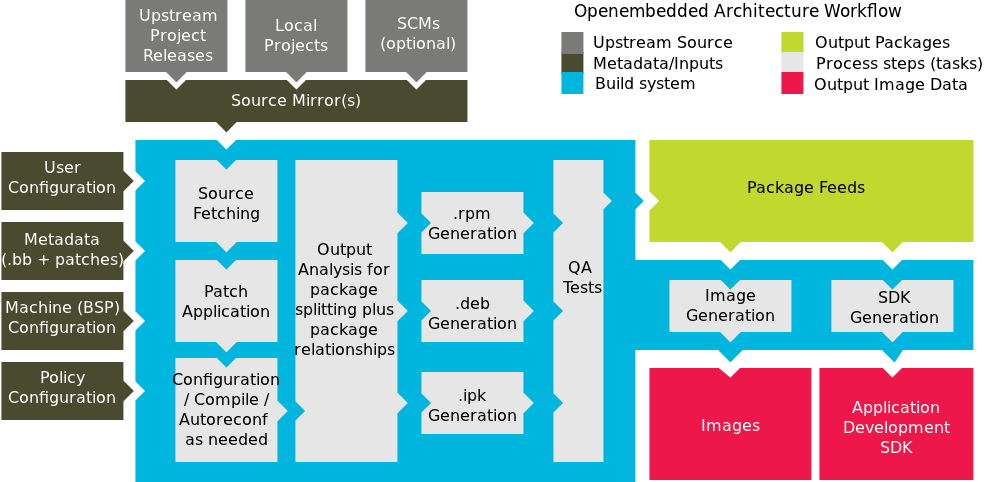
\includegraphics[width=8cm]{yocto-environment.png}
\end{frame}

\begin{frame}
  \frametitle{Основные типы файлов метаданных}
  \begin{itemize}
    \item \textbf{.bb} -- рецепт bitbake 
    \item \textbf{.bbappend} -- модификации существующих рецептов bitbake 
    \item \textbf{.conf} -- конфигурационные файлы (установка переменных)
    \item \textbf{.bbclass} -- определение команд, используемых в рецептах 
  \end{itemize}
\end{frame}

\begin{frame}
  \frametitle{Композиция слоев: абстрактная борда в вакууме}
  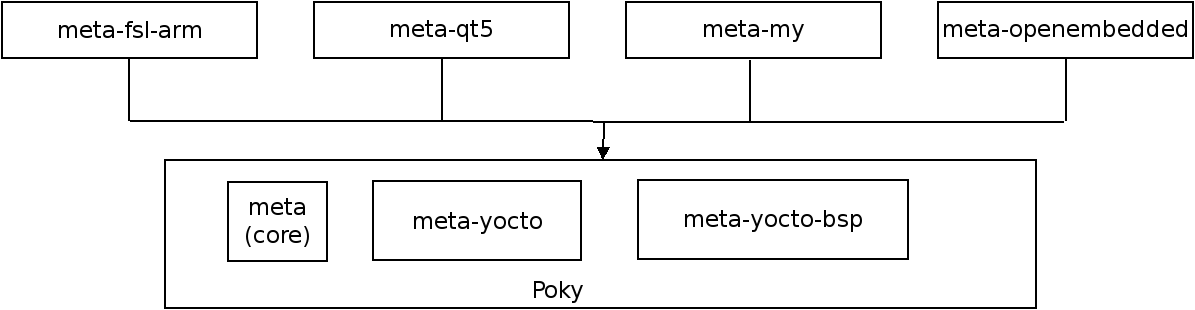
\includegraphics[width=8cm]{yocto-basic-meta.png}
\end{frame}

\begin{frame}
  \frametitle{Композиция слоев: raspberry pi}
  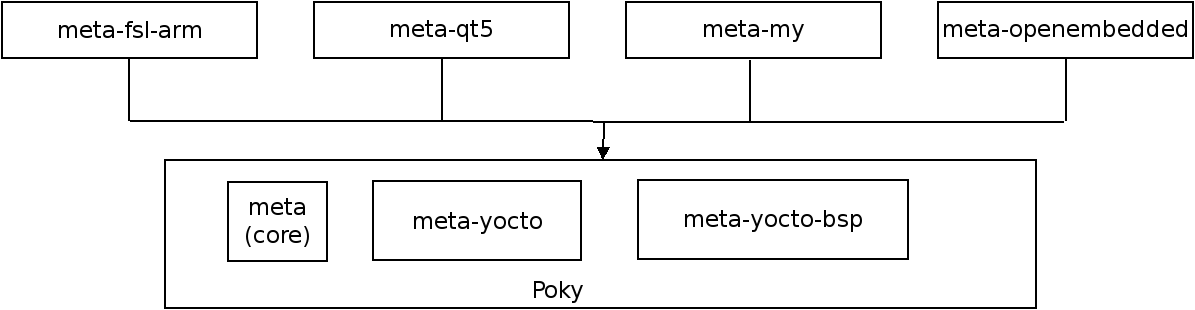
\includegraphics[width=8cm]{yocto-basic-meta.png}
\end{frame}

\subsection{Сборка для raspberry pi}
\begin{frame}[fragile]
  \frametitle{Минимальная прошивка: добыча пакетов}
\begin{lstlisting}[language=bash]
git clone git://git.yoctoproject.org/poky.git -b rocko
git clone git://git.yoctoproject.org/meta-openembedded.git -b rocko
git clone git://git.yoctoproject.org/meta-raspberrypi.git -b rocko
\end{lstlisting}
\end{frame}

\begin{frame}[fragile]
   \frametitle{Минимальная прошивка: конфигурация}
\begin{lstlisting}[language=bash]
source poky/oe-init-build-env rpi-build # настройка окружения
cd rpi-build # rpi-build -- директория для сборки
\end{lstlisting}
  \begin{itemize}
    \item Отредактировать \texttt{conf/bblayers.conf}
    \item Отредактировать \texttt{conf/local.conf}
    \item Инструкции смотреть в файле meta-raspberrypi/README.md
  \end{itemize}
\begin{lstlisting}[language=bash]
bitbake rpi-hwup-image
\end{lstlisting}
\end{frame}

\begin{frame}
  \frametitle{Структура директорий после сборки}
  Корень --build директория, в нашем случае rpi-build
  \begin{itemize}
    \item \texttt{conf} Директория с настройками
    \item \texttt{downloads} Исходники пакетов
    \item \texttt{tmp} Результаты сборки
    \begin{itemize}
       \item \texttt{deploy/images} Образы для заливки
       \item \texttt{deploy/rpm} Файлы пакетов для пакетного менеджера
    \end{itemize}
  \end{itemize}
\end{frame}

\subsection{Добавление своих рецептов}

\begin{frame}
  \frametitle{Структура директорий метаслоя}
  \begin{itemize}
    \item \texttt{conf}
      \begin{itemize}
          \item \texttt{layer.conf}
      \end{itemize}
    \item \texttt{recipes-mypackages}
      \begin{itemize}
        \item \texttt{example}
          \begin{itemize}
            \item \texttt{example\_0.1}
             % \begin{itemize}
                \item \texttt{--- hello.c}
             % \end{itemize}
          \end{itemize}
          \item \texttt{example\_0.1.bb}  - рецепт
      \end{itemize}
  \end{itemize}
\end{frame}

\begin{frame}[fragile]
  \frametitle{Файл layer.conf}
\begin{lstlisting}[language=make]
BBPATH .= ":${LAYERDIR}"

BBFILES += "${LAYERDIR}/recipes-*/*/*.bb \
            ${LAYERDIR}/recipes-*/*/*.bbappend"

BBFILE_COLLECTIONS += "my"
BBFILE_PATTERN_my = "^${LAYERDIR}/"
BBFILE_PRIORITY_my = "6"
\end{lstlisting}
\end{frame}

\begin{frame}[fragile]
  \frametitle{Рецепт}
\begin{lstlisting}[language=make]
DESCRIPTION = "..."
SECTION = "examples"
LICENSE = "GPLv2"
LIC_FILES_CHKSUM = "file://${COMMON_LICENSE_DIR}/GPLv2;md5=..."
PR="r0"

SRC_URI = "file://hello.c"

S = "${WORKDIR}"

do_compile() {
   ${CC} hello.c -o hello
}

do_install () {
  install -d ${D}${bindir}
  install -m 0755 hello ${D}{bindir}
}
\end{lstlisting}
\end{frame}

\begin{frame}[fragile]
  \frametitle{}
\end{frame}
\end{document}
